\documentclass{beamer}
\usetheme{default}
\usecolortheme{seahorse}
\usepackage[utf8]{inputenc}
\usepackage{graphicx}
\usepackage{booktabs}
\usepackage{amsmath}
\usepackage{natbib}
\usepackage[english]{babel}
\usepackage{hyphenat}
\usepackage{tikz}
\usetikzlibrary{shapes,arrows.meta,positioning}

\title[Lecture 1]{Hello, Psychometrics!}
\subtitle{Advanced Master in Agricultural Economics and Policy}
\author{Giovanbattista Califano}
\date[Portici, 20/04/2026]{Attitudinal Scales for the Study \\ of Consumer Preferences \\ April 20, 2026}
\institute[UNINA]{University of Naples Federico II, giovanbattista.califano@unina.it}

\AtBeginSection[]
{
  \begin{frame}<beamer>
    \frametitle{Moving on to...}
    \tableofcontents[currentsection]
  \end{frame}
}

\begin{document}

\frame{\titlepage}

\begin{frame}{Roadmap}
    \begin{center}
        \begin{tabular}{|l|l|c|}
        \hline
        20/04 &  Hello, Psychometrics! & $\bigcirc$ \\
        \hline
        23/04 &  The Questionnaire & $\bigcirc$ \\
        \hline
        24/04 & Reliability and Validity of a Measure & $\bigcirc$ \\
        \hline
        27/04 & Latent Variables: Reflective or Formative? & $\bigcirc$ \\
        \hline
        30/04 & A Bit of SEM & $\bigcirc$ \\
        \hline
        07/05 & Stata Stata Stata Stata Stata Stata Stata & $\bigcirc$ \\
        \hline
        \end{tabular}
    \end{center}
\vspace{0.1cm}
\footnotesize
Recommended readings: \\
\begin{itemize}
    \item Chapters 4 and 7 from \cite{jhangiani2019research}
    \item Chapters 7, 10 and 14 from \cite{olivero2022psicologia}
    \item Chapter 12 from \cite{mehmetoglu2022applied}
\end{itemize}
\scriptsize
\bibliographystyle{apalike}
\bibliography{text}
\end{frame}

\begin{frame}{Why psychometrics? The case of Dr. Mirko Marmellata}
\begin{figure}
    \centering
    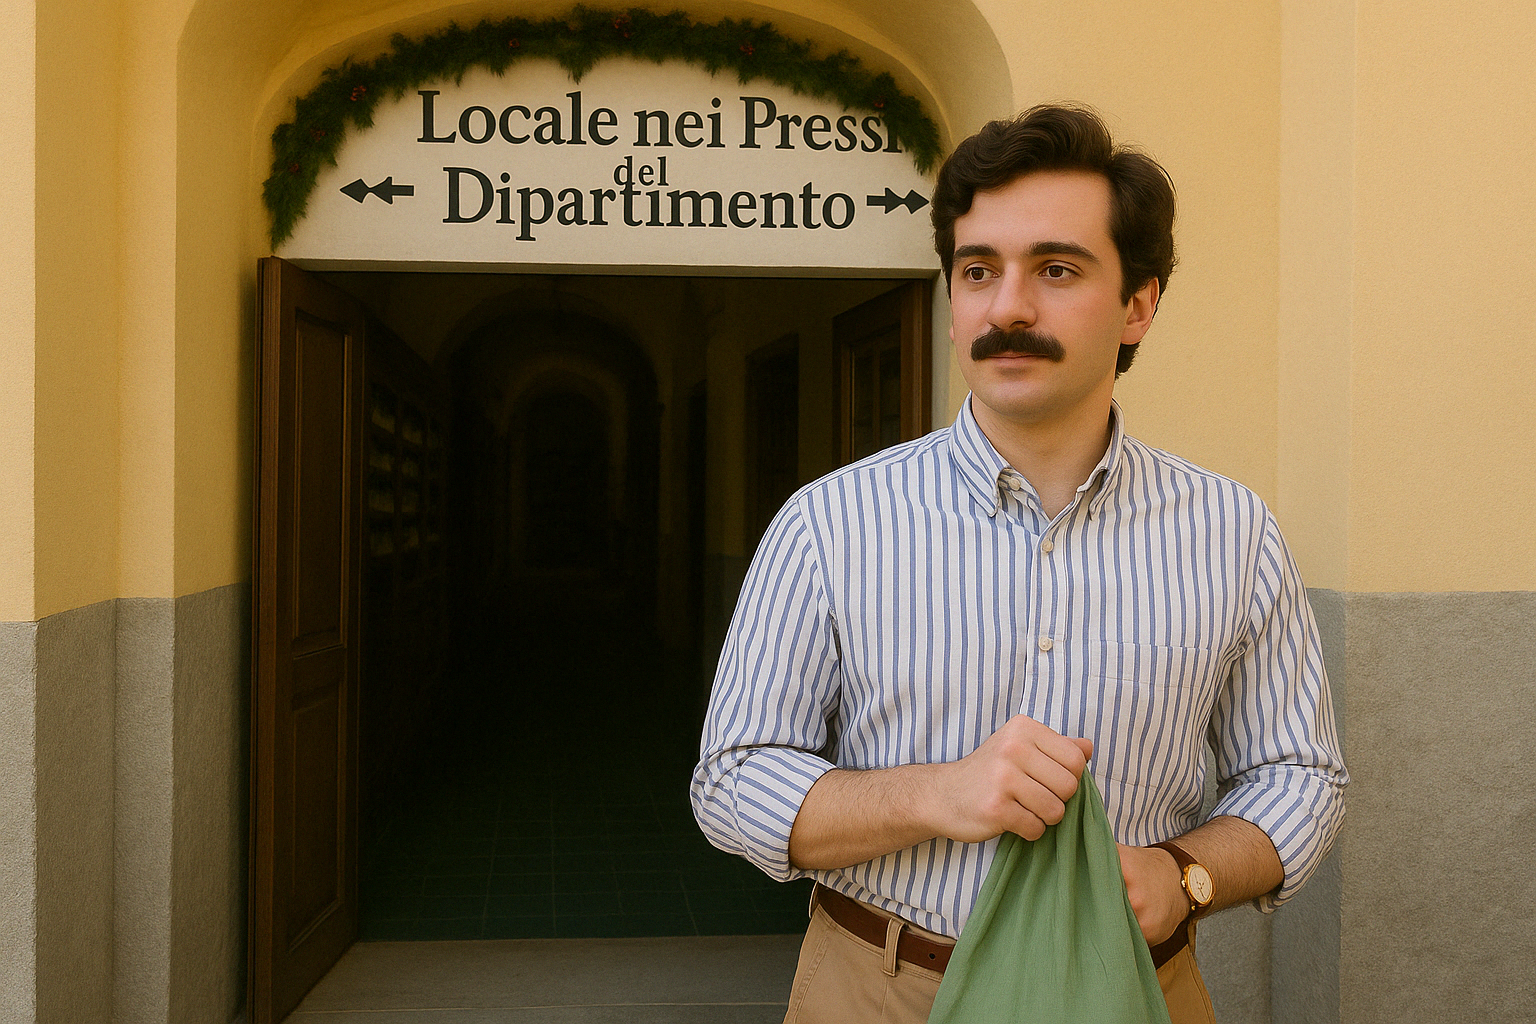
\includegraphics[width=\linewidth]{mirko.png}
\end{figure}
\end{frame}

\begin{frame}{Why psychometrics? The case of Dr. Mirko Marmellata}
\begin{block}{Dr. Marmellata}
every day chooses to buy lunch at the \textit{Local Restaurant Near the Department}, despite spending much more than bringing lunch from home, and never being fully satisfied with the quality and quantity offered.
\end{block}
\vspace{1em}
\begin{block}{By the standards of homo oeconomicus}
his choice would be \textbf{irrational}. To be fair, the choice still appears to us as \textbf{suboptimal}.
\end{block}
\end{frame}

\begin{frame}{Why psychometrics? The case of Dr. Mirko Marmellata}
\begin{block}{Random Utility Model (RUM)}
\[
U_{ia} = V_{ia} + \varepsilon_{ia}
\]
\begin{itemize}
  \item \(U_{ia}\): total utility that individual \(i\) associates with alternative \(a\);
  \item \(V_{ia}\): observable component (price, quantity...);
  \item \(\varepsilon_{ia}\): unobserved component (habits, emotions...).
\end{itemize}
\end{block}
\vspace{1em}
\begin{block}{For Mirko Marmellata:}
\[
U_{\text{MM}, \text{Restaurant}} > U_{\text{MM}, \text{Home}}
\]
What drives his preference is probably hidden in \(\varepsilon\).
\end{block}
\end{frame}

\begin{frame}{Why psychometrics? The case of Dr. Mirko Marmellata}
\begin{block}{The role of psychometrics}
It allows us to ``open'' the \(\varepsilon\) and model the latent constructs that influence decisions.
\end{block}
\vspace{1em}
\begin{block}{Objective}
To bring psychological factors out of \(\varepsilon\) and into the model, improving \textbf{prediction} and \textbf{understanding}.
\end{block}
\end{frame}

\section{Brief Introduction to Measurement Theory}
\begin{frame}{Vietnam flashback...}
\begin{center}
   {\huge \alert{DATA GENERATING PROCESS}}
\end{center}
\vspace{0.5cm}
\begin{itemize}
    \item How do we measure something we cannot observe?
\end{itemize}
\pause
\vspace{0.5cm}
According to \textbf{measurement theory}, even if we cannot directly observe a theoretical concept (such as intelligence), we can observe its {\it reflections} in reality: behaviours, responses, outcomes... \\
\vspace{0.5 cm}
\footnotesize
{\it Example:} \\
We do not weigh a person's intelligence on a scale, but we can infer it from a series of signals: they graduated with honours, they are good at Stata, they use complex words, they have read all the nineteenth-century Russian novels... {\it Note that a lot depends on our definition of intelligence!}
\end{frame}

\begin{frame}{What we mean by measurement}
\begin{block}{Proposed definition:}
    The \textit{systematic} assignment of a score to entities (individuals, objects, events...), such that the score represents a characteristic of those entities.
\end{block}
\pause
\begin{itemize}
    \item When the characteristic under investigation is psychological in nature, the science of measurement is called \textbf{psychometrics}.
\end{itemize}
\end{frame}

\section{Constructs: Conceptual and Operational Definitions}
\begin{frame}{Constructs}
Some characteristics of interest are simple to measure: the consumer's age, height, weight. \\ Others, such as intelligence, self-esteem or attitudes, cannot be directly observed.
\begin{itemize}
    \item These variables are called \textbf{constructs}.
\end{itemize}
\end{frame}

\begin{frame}{Constructs}
Constructs include (but are not limited to):
    \begin{itemize}
      \item Personality traits (e.g. extraversion)
      \item Emotional states (e.g. fear)
      \item Attitudes (e.g. towards certifications)
      \item Abilities (e.g. in scientific subjects)
    \end{itemize}
\end{frame}

\begin{frame}{Constructs}
  \begin{itemize}
    \item The construct describes a \textit{general tendency} to act in a certain way, not a specific behaviour at a given moment.
    \item Constructs are \textbf{abstract summaries} of complex processes.
    \item No single behaviour or process can fully ``define'' the construct.
  \end{itemize}
\end{frame}

\begin{frame}{Conceptual definition of a construct}
  \begin{block}{What is a conceptual definition?}
    It describes the behaviours and internal processes that constitute a psychological construct, and explains how it relates to other variables.
  \end{block}
  \pause
  \begin{itemize}
    \item Example: \textbf{neuroticism} can be defined as the stable tendency to experience negative emotions (anxiety, anger, sadness) across multiple situations.
    \item It may also include: genetic origins, stability over time, correlations with physical pain and somatic symptoms.
    \pause
    \item Scientific definitions differ from dictionary definitions (more precise, empirically testable, and open to revision).
    \item Often multiple conceptual definitions of the same construct exist in the literature.
  \end{itemize}
\end{frame}

\begin{frame}{Operational definition of a construct}
  \begin{block}{What is an operational definition?}
    It is a definition of a construct in terms of how it is concretely measured.
  \end{block}
  \pause
\vspace{0.8cm}
  \begin{center}
      \textbf{Conceptual definition} \\
      \bigskip
      $\Downarrow$ \quad \textit{\small Operationalisation} \quad $\Downarrow$ \\
      \bigskip
      \textbf{Operational definition} \\
  \end{center}
\end{frame}


\begin{frame}{Operational definition of a construct}
  Operational measures fall into three broad categories:
  \begin{enumerate}
      \item \textbf{Self-report}: the individual reports their own thoughts, emotions or behaviours.
      \item \textbf{Behavioural}: a behaviour is observed and recorded.
      \item \textbf{Physiological}: biological processes are recorded.
    \end{enumerate}
\end{frame}

\begin{frame}{Example: Disgust response towards an "expired" yoghurt}
\small
  Suppose we want to measure the \textbf{disgust} reaction of a consumer towards a yoghurt that has passed its best-before date.
  \pause
      \begin{block}{Conceptual definition}
    Disgust is a basic emotion manifested as an avoidance response to stimuli perceived as contaminating, infected or degraded. It has an evolutionary function of protecting against the ingestion of potentially harmful substances.
  \end{block}
  \pause
    \begin{block}{Operational definitions}
  \begin{itemize}
    \item \textbf{Self-report}: the participant rates how disgusting they find the idea of tasting the product on a scale from 1 to 7.
    \item \textbf{Behavioural}: it is observed whether the participant refuses to taste the product.
    \item \textbf{Physiological}: the galvanic skin response (GSR) or facial muscle activity (EMG) related to disgust is measured when the participant is asked to taste the product.
  \end{itemize}
\end{block}
\end{frame}

\section{Levels of Measurement}
\begin{frame}{Levels of measurement}
  \begin{block}{The level of measurement can be:}
    \begin{enumerate}
      \item Nominal
      \item Ordinal
      \item Interval
      \item Ratio
    \end{enumerate}
 \end{block}
Each level conveys a different degree of quantitative information, and determines the appropriate statistical analyses.
\end{frame}

\begin{frame}{Nominal and Ordinal}
\begin{block}{Nominal}
    Category labels: e.g. gender, marital status, ethnicity, favourite colour. \textbf{There is no order among the categories.}
\end{block}
\pause
\begin{block}{Ordinal}
    The categories have an order (e.g. "very satisfied", "satisfied", "dissatisfied") \textbf{but it is not possible to assume that the distances between categories are equal.} \\
    \pause
    \centering
    \vspace{0.5em}
    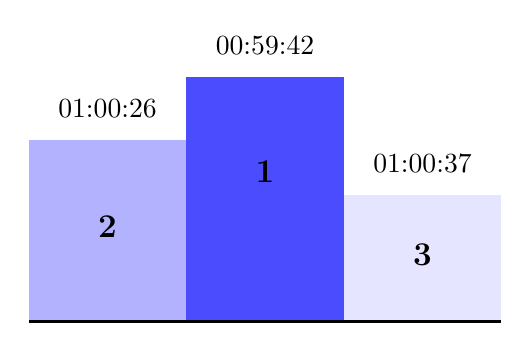
\begin{tikzpicture}[x=2cm,y=1cm]
  \fill[blue!30] (-1,-0.1) rectangle (0,2.2);
  \fill[blue!70] ( 0,-0.1) rectangle (1,3.0);
  \fill[blue!10] ( 1,-0.1) rectangle (2,1.5);
  \node[font=\large\bfseries] at (-0.5,1.1) {2};
  \node[font=\large\bfseries] at ( 0.5,1.8) {1};
  \node[font=\large\bfseries] at ( 1.5,0.75) {3};
\draw[thick] (-1,-0.1) -- (2,-0.1);
    \pause
  \node at (-0.5,2.6) {01:00:26};
  \node at ( 0.5,3.4) {00:59:42};
  \node at ( 1.5,1.9) {01:00:37};
\end{tikzpicture}
\end{block}
\end{frame}

\begin{frame}{Interval and Ratio}
  \begin{block}{Interval}
  Numerical differences with consistent meaning: e.g. degrees Celsius. \\
  The distance between 12°C and 22°C is the same as that between 22°C and 32°C. However...
    \begin{itemize}
      \item \textbf{No true zero:} 0°C does not mean ``absence of temperature''.
      \item Therefore \textbf{it makes no sense to speak of ``double'' or ``half'':} at 30°C it is not twice as hot as at 15°C.
    \end{itemize}
  \end{block}
  \pause
  \begin{block}{Ratio}
  Like interval, but with zero indicating the \textbf{absolute origin}. \\
    \begin{itemize}
      \item Allows proportional comparisons: 100 kg is twice 50 kg.
      \item E.g.: height, weight, income, temperature in Kelvin.
    \end{itemize}
  \end{block}
\end{frame}

\begin{frame}{Summary}
    \centering
    Possible operations with the different measurement scales: \\
    \vspace{1em}
    \begin{tabular}{lcccc}
    \toprule
      \textbf{Level} & \textbf{$=$ $\neq$} & \textbf{$>$ $<$} & \textbf{$+$ $-$} & \textbf{$\times$ $\div$} \\
      \midrule
      Nominal & \checkmark & & & \\
      Ordinal & \checkmark & \checkmark & & \\
      Interval & \checkmark & \checkmark & \checkmark & \\
      Ratio & \checkmark & \checkmark & \checkmark & \checkmark \\
      \bottomrule
    \end{tabular}
\end{frame}
\end{document}
